\chapter{UI Construction}\label{ch01:03}

%\section{UX with TG}

%\section{How to Swing}

%\section{Property Editors}

%\section{Entity Grid Inspector}

%\section{Actions in action}

%\section{Trees as Menus}

%\section{Constructing Entity Centres}

\section{Constructing Entity Masters}

  The notion of an \emph{entity master} refers to UI that provides a way of creating new and modifying existing entity instances.
  Regardless of its complexity, all entity masters contain property editors and a predefined set of actions such as \emph{New}, \emph{Edit}, \emph{Save}, \emph{Cancel} and \emph{Refresh}.
  The type and behaviour of property editors depends on the type the associated with them entity properties.
  Thus, during development we do not directly work with UI components, but instead with their abstractions, referring to them by property name.
  For example, having a UI model (this is discussed a bit farther in the text) we can simply request a collection of all property editors for an entity instance.
  
  The resultant collection would contain UI controls that are bound to properties of a corresponding entity instance.
  This way any change to the property value by user from UI gets automatically propagated to the property via its setter, validation mechanism etc.
  And vice versa, any programmatic change to the property by invoking its setter gets automatically reflected in the UI.
  Listing~\ref{lst:PropertiesMap} illustrates a process of obtaining an instance of \texttt{IPropertyEditor} by property name, and access to the actual underlying Swing component that represents the editor from UI perspective.
  Naturally, the obtained editor can be added to some UI container such as \texttt{JPanel} or \texttt{JFrame}.
  This approach streamlines UI development to the task of component layouting, which will be discussed later in this chapter in greater detail.
  
  
  \lstset{language=Java,
	  escapechar=\%,
	  numbers=left, numberstyle=\tiny, basicstyle=\scriptsize\color{basiccolor}, stepnumber=1, numbersep=5pt, keywordstyle=\bfseries\color{codefgcolor}, stringstyle=\color{stringcolor}}
  \begin{code}{One-to-One association.}{\label{lst:PropertiesMap}}{codebgcolor}
    \begin{lstlisting}
    ...
IPropertyEditor myPropertyEditor = model.getEditors().get("myProperty");
JComponent actualComponent = myPropertyEditor.getEditor();
    ...
    \end{lstlisting}
  \end{code}
  
  
  Each entity object, if required to be created or changed, should be provided with its own entity master implementation. 
  An instance of \texttt{EntityMasterManager} should be created at the client application startup time, which should be used for obtaining an instance of entity master by an instance of entity object.
  It ensures that only one instance of entity master exists for any particular instance of an entity object, and either creates a new entity master instance or brings to front and existing one when handling a request to show an entity master.
  
  As a convenience, the application template generated by Maven archetype, provide class \texttt{EntityMasterManagerConfig} with method \texttt{createEntityMasterFactory} that produces an instance of \texttt{EntityMasterManager}.
  Therefore, if an entity master is created it only needs to be associated with a corresponding entity type in order to get wired into the UI framework (this, for example, allow calling masters by means of double-click on entities in Entity Centres etc.).
  
  As mentioned in previous chapters, the platform employs the Model-View-Presenter (MVP) pattern for building UI.
  Thus, each entity master has at least one model and a view associated with that model.  
  In order to automate the routine task of creating UI, the platform offers a number of UI models that can be used as the basis for building custom, entity specific models and views.
  The rest of the chapter discusses specific models and their application for building simple and compound entity masters.
  
\subsection{Simple Masters}
  Simple master refers to masters for simple entities that may fit editors for all their properties on a single view such as panel.
  Simple entities often model so called \emph{reference data} or \emph{table codes}.
  Often such entities have just a handful of properties that can be conveniently represented on a single view.
  That's where simple masters are applicable.
  
  Structurally, simple master consists of four main components:
  
  \begin{description}
   \item[\textbf{Model.}] A class, usually derived from \texttt{UmMasterWithCrudAndUpdater<EntityObjectType, EntityCompanionType>}, representing UI model for the master.
   Here \texttt{Um} stands for \emph{UI Model}, \texttt{CrudAndUpdater} indicates that model provide essential CRUD operations with feedback loop to the view (this is the updater part).
   The first type parameter is an entity object type the model is designed for, the second -- a type of a corresponding companion object.
   Both entity and companion objects are passed into the model's constructor.
   \item[\textbf{View.}] A class, usually derived from \texttt{BaseNotifPanel<UmMasterType>}, which represents a container holding property editors, the action buttons and the notification panel at the top. 
   It specifies what UI master model it expects at type parameter and requires for the model instance to be provided into its constructor. 
   This is where developers define the layout of property editors on the master.
   \item[\textbf{Frame.}] This is really just a class, usually derived from \texttt{BaseFrame}, that holds the view as on its own it cannot be displayed.   
   \item[\textbf{Factory.}] A descendent from \texttt{IEntityMasterFactory<Entity\-Object\-Type, Entity\-Companion\-Type>} responsible for master instantiation.   
   It is used by the internal platform mechanism to instantiate entity masters.
  \end{description}
  

  \subsubsection{Model}
  
  The \textbf{model} is the central component of the master structure. 
  All other components revolve around it.  
  Here we specifically discuss the model base class \texttt{UmMasterWithCrudAndUpdater}.
  
  The following list specifies the major pieces required for model construction.
  These pieces are passed into the model's class constructor.
  \begin{description}
   \item[\textbf{Entity producer.}] An instance of a class implementing contract \texttt{IEntityProducer<EntityObjectType>}.
   It is responsible for creation of new entity object instances, which happens when user chooses action \emph{New}.
   This contract provides a convenient way to abstract specific details of entity instantiation away from UI code.
   Each entity object type should have its own producer implementation, which gets registered with \texttt{EntityMasterManager}.
   If custom instantiation is not required then a default producer provided automatically without the need to register it.
   \item[\textbf{Cache.}] An instance of a class implementing contract \texttt{IEntityMasterCache} that represents a global cache for all master instances for different entity objects.
   A default cache implementation is provided automatically and requires no action from developers to use it.
   It could be argued in such case there is no need to expose it, but we felt that it is always good to provide extension points with reasonable defaults.
   Thus, a custom case implementation can be provided in case the default is not sufficient.
   The client-side application IoC module controls the biding of the \texttt{IEntityMasterCache} contract.
   \item[\textbf{Entity object.}] An instance of an entity object for which the master is being created.
   For the very least entity id should be present in this instance.
   \item[\textbf{Companion object.}] An instance of a companion object of the entity for which the master is being created.   
   \item[\textbf{Entity object fetch model.}] An instance of \texttt{fetch<EntityObjectType>} that defines what entity properties and subproperties should be fetched when obtaining entity instance from the database.
   \item[\textbf{Property binder.}] An instance of class \texttt{MasterPropertyBinder<EntityObjectType>} responsible for binding logic between property editors and properties.
   The platform provide convenient factory methods to streamline creation of binders.
   \item[\textbf{Lazy initialisation.}] A boolean argument that specifies whether property editors should be created and bound at the time of model instantiation (value \emph{true}) or at some later stage (value \emph{false}).
   For relatively simple masters this value can safely be set to \emph{false}.
   \item[\textbf{View owner.}] All entity masters are created as a user action on an entity centre.
   This makes entity centres act like the owners of the produced from them masters.
   Theoretically there could be other kinds of master owners.
   Therefore, the master ownership is abstracted into contract \texttt{IUmViewOwner}.
   Naturally entity centres implement this contract.
   It has only one method \texttt{notifyEntityChange}, which is invoked when entity is modified on the master.
   This provides a convenient way for the owner to react to the entity modification (e.g. entity centres update the row in the resultant grid corresponding to the entity instance).
   \item[\textbf{Frame title updater.}] A frame title bar is a convenient place for providing information about the master's state or related events.
   Neither model nor view has any knowledge of the intended parent where it would be placed such as another view or a frame.
   Therefore, there is a need to have a mechanism that could update a title bar.
   This need is realised by providing an instance of \texttt{FrameTitleUpdater}, which takes frame as its construction argument.
   This way, the logic in the model can invoke method \texttt{update(String)} any time frame's title needs to be update.
   Method \texttt{update(String)} runs on Event Dispatch Thread (EDT) and thus can be invoked from any other thread that might be performing some business logic.   
  \end{description}
  
  Property binder depends on \emph{value matcher factory} (\texttt{IValueMatcherFactory}) to provide value matcher for autocompleters, \emph{master manager} (\texttt{IMasterDomainTreeManager}) to persist user-defined autocompleter configuration and \emph{criteria generator} (\texttt{ICriteriaGenerator}) to handle  user-defined autocompleter configuration queries.
  All these dependencies have default IoC bindings and can be easily obtained when creating property binders.
  
  It is important to understand that models should not contain any business logic.
  Basically, the main responsibility of any model is to serve as a glue that binds together UI with the business logic implemented as part of entity companion object.
  The model provides actions (as in \texttt{javax.swing.Action} implementation) \texttt{newAction}, \texttt{editAction}, \texttt{saveAction}, \texttt{cancelAction}, \texttt{deleteAction} and \texttt{refreshAction} to support CRUD operations.
  Respective getters should be used when composing an action panel with buttons in a corresponding view.
  Custom action can be provided by developers.
  
  An essential part of the model concept is its \emph{state} and \emph{action stage}.
  The change in state can be caused by user or programmatical calls of CRUD actions.
  Custom actions should also maintain the state.
  The sate is represented by enumeration \texttt{UmState} and is set be invoking method \texttt{setSate(UmState)} on the model.
  The following state are available:
  \begin{description}
    \item[\textbf{VIEW}] -- indicates that model is in review state of an existing entity object; this is the default state; no properties can be changed.
    \item[\textbf{EDIT}] -- indicates that model is in editing state; property editors are enabled and user may change property values.
    \item[\textbf{NEW}] -- indicates that model is editing state, but for a brand new entity object that gets created as the result of calling \texttt{newAction}.    
    \item[\textbf{UNDEFINED}] -- indicates that the model is in transition between states and one of the other states will be reached soon.    
    \item[\textbf{CUSTOM}] -- a state that should be used in conjunction with custom actions; its effect is similar to EDIT or NEW in a way that internally the UI model considers this as \emph{unsaved} mode.
  \end{description}
    
  Due to the fact that change in state is always the result of some action (either CRUD or custom), a mechanism for observing actions' execution stages is provided in order to support handling of state transition at fine grained level.
  Specifically, each supported out of the box action updates its execution stage during execution.
  Each action (including custom) has three stages:
  \begin{description}
    \item[\textbf{PRE\_ACTION}] -- refers to the stage where action is preparing to execute (e.g. initialises a blocking layer).
    \item[\textbf{ACTION}] -- refers to the stage where action is executing.
    \item[\textbf{POST\_ACTION}] -- refers to the stage where action finished its task and performs some post action activities (e.g. releases a blocking layer)
  \end{description}
  
  For example, the three states for action \texttt{newAction} are \texttt{NEW\_PRE\_ACTION}, \texttt{NEW\_ACTION} and \texttt{NEW\_POST\_ACTION}.
  Custom actions should use stages \texttt{CUSTOM\_PRE\_ACTION}, \texttt{CUSTOM\_ACTION} and \texttt{CUSTOM\_POST\_ACTION}. 
  For more stages refer enumerations \texttt{UModel.ActionStage}.
  
  In order to react to state change, model's method \texttt{notifyActionStageChange(ActionStage)} should be overridden and custom logic provided.
  An example of this method overridden implementation to focus a property editor when \texttt{editAction} finishes its execution, is provided in listing~\ref{lst:EDIT_POST_ACTION_handling}.
  
  \begin{code}{EDIT\_POST\_ACTION handling.}{\label{lst:EDIT_POST_ACTION_handling}}{codebgcolor}
    \begin{lstlisting}
...    
@Override    
protected void notifyActionStageChange(final ActionStage actionState) {
  super.notifyActionStageChange(actionState);%\tikzref{lst_EDIT_POST_ACTION_handling_1}{0.1cm}{0.1cm}%
 
  if (actionState == ActionStage.EDIT_POST_ACTION) { %\tikzref{lst_EDIT_POST_ACTION_handling_2}{0.1cm}{0.1cm}%
    getEditors().get("desc").getEditor().requestFocusInWindow();
  }
}
...
    \end{lstlisting}
  \end{code}
  \tikznote{lst_EDIT_POST_ACTION_handling_1_annotation}{lst_EDIT_POST_ACTION_handling_1}{2cm}{0.8cm}{7cm}
    {Super}
    {Inherited handling might do some useful work, thus invoking it.}    
  \tikznote{lst_EDIT_POST_ACTION_handling_1_annotation}{lst_EDIT_POST_ACTION_handling_2}{3cm}{-1.1cm}{5cm}
    {EDIT\_POST\_ACTION}
    {Check if the this is the stage that needs to be handled. If so then obtain editor for property \emph{desc} and focus it.}
  
  The last important item to conclude UI model discussion, is the notion of \emph{managed entity}.
  Basically, an entity object instance that is associated with master is considered to be managed by the model.
  It can be obtained by calling method \texttt{getManagedEntity()}.
  From the developer perspective, the managed entity is fully controlled from within the model and there is no way to set it into the model except at the time of model creation.  
  
  \paragraph{Model Example}
  
  In order to provide a complete example, let's consider our Rail domain.
  One of the important business entities in this domain is \emph{Workshop}.
  This entity has a companion object \emph{IWorkshop}.
  At this stage it is not important what properties entity object Workshop has, but we can assume that it has at least properties \texttt{key} and \texttt{desc}.
  
  One possible way to implement workshop UI model is presented in listing~\ref{lst:workshop-ui-model}.
  The provided callouts describe each section on the model.
  
  
  \begin{code}{Workshop UI model.}{\label{lst:workshop-ui-model}}{codebgcolor}
    \begin{lstlisting}
public class WorkshopMasterModel 
    extends UmMasterWithCrudAndUpdater<Workshop, IWorkshop> {%\tikzref{lst_workshop-ui-model-1}{-2.5cm}{0.2cm}%

    private final static fetch<Workshop> qm = fetchAll(Workshop.class);%\tikzref{lst_workshop-ui-model-2}{-0.5cm}{0.2cm}%
    
    public WorkshopMasterModel(//
    	final IEntityProducer<Workshop> entityProducer,//
    	final IEntityMasterCache cache,//
    	final Workshop entity,//
    	final IWorkshop controller,//
    	final IValueMatcherFactory valueMatcherFactory,//%\tikzref{lst_workshop-ui-model-3}{0.1cm}{0.2cm}%
    	final IUmViewOwner owner,//
    	final FrameTitleUpdater titleUpdater,//
    	final IMasterDomainTreeManager masterManager,//
    	final ICriteriaGenerator criteriaGenerator) {
        super(entityProducer, cache, entity, controller, //%\tikzref{lst_workshop-ui-model-4}{1.2cm}{-0.1cm}%
              MasterPropertyBinder.<Workshop> createPropertyBinderWithLocatorSupport(//
     			valueMatcherFactory, //
     			masterManager, //
     			criteriaGenerator),//
     	     qm, titleUpdater, owner, false);%\tikzref{lst_workshop-ui-model-5}{0.2cm}{0.2cm}%
        setState(UmState.VIEW);%\tikzref{lst_workshop-ui-model-6}{0.1cm}{0.0cm}%
    }
     
    @Override
    protected void notifyActionStageChange(final ActionStage actionState) {
        super.notifyActionStageChange(actionState);
        if (actionState == ActionStage.EDIT_POST_ACTION) {%\tikzref{lst_workshop-ui-model-7}{0.1cm}{0.1cm}%            
            getEditors().get("desc").getEditor().requestFocusInWindow();
         }
    }
     
    @Override
    public String toString() {
        return "Workshop Master";%\tikzref{lst_workshop-ui-model-8}{0.1cm}{0.1cm}%            
    }
     
    @Override
    protected String defaultTitle() {
        return toString();
    }
}
    \end{lstlisting}
  \end{code}
  \tikznote{lst_workshop-ui-model_1-annotation}{lst_workshop-ui-model-1}{2cm}{0.8cm}{6.5cm}
    {Supermodel Parameters}
    {Type parameters indicate that model is for entity Workshop.}
  \tikznote{lst_workshop-ui-model_2-annotation}{lst_workshop-ui-model-2}{3cm}{0.2cm}{4cm}
    {Fetch model}
    {The fetch model states that all workshop properties should be fetched for the master to function.}
  \tikznote{lst_workshop-ui-model_3-annotation}{lst_workshop-ui-model-3}{3cm}{0.2cm}{4cm}
    {Constructor Arguments}
    {All formal arguments are listed as discussed above.}
  \tikznote{lst_workshop-ui-model_4-annotation}{lst_workshop-ui-model-4}{2cm}{0.7cm}{5cm}
    {Property Binder}
    {Creation of the binder for producing property editors.}
\tikznote{lst_workshop-ui-model_5-annotation}{lst_workshop-ui-model-5}{3cm}{0.2cm}{4cm}
    {Non-lazy}
    {Argument false indicates non-lazy initialisation, and thus all property editors are created as part of model instantiation.}
\tikznote{lst_workshop-ui-model_6-annotation}{lst_workshop-ui-model-6}{3cm}{-0.4cm}{4cm}
    {Model state}
    {The state of the model is set to VIEW.}
\tikznote{lst_workshop-ui-model_7-annotation}{lst_workshop-ui-model-7}{3cm}{0.5cm}{4cm}
    {Action stage change handler}
    {When user invokes the edit action, the editor for property \texttt{desc} gets focused.}
\tikznote{lst_workshop-ui-model_8-annotation}{lst_workshop-ui-model-8}{3cm}{0.5cm}{4cm}
    {View title}
    {The view title should also be driven by model. This way there is always one place too look for UI definitions.}
    
  
  \subsubsection{View}
  
  The \emph{view} concept has a single responsibility -- visualisation of entity state and provide access to actions applicable to that entity.
  Every view is associated with a model, which is passed into view's class constructor.
  Views should have neither UI nor business logic in them.
  All UI logic should be localised in a corresponding model and the view simply taps into it.
  
  In its simplest form, which is the case in this context, views are panels responsible only for layouting property editors and buttons linked to appropriated actions.
  Both property editors and actions can be obtained from the model.  
  It is recommended to subclass \texttt{BaseNotifPanel<UI Model Type>} when creating views.
  This base class provides convenient features, including a number of methods for layouting UI controls based on MigLayout manager.
  MigLayout is the recommended and expected layout manager to be used for building view~\cite{MigLayout}.
  Listing~\ref{lst:view_example} provides a view example for entity \emph{Workshop}, which is based on the earlier introduced model \emph{WorkshopMasterModel}.
  Let's discuss it in details.  
  
    \begin{code}{View example.}{\label{lst:view_example}}{codebgcolor}
    \begin{lstlisting}
public class WorkshopMasterView extends BaseNotifPanel<WorkshopMasterModel> {    

    public WorkshopMasterView(final WorkshopMasterModel model) {
	super(model.toString(), model);
	final JPanel componentsPanel = new JPanel(new MigLayout("insets 0", 
	     "[:50:][grow,fill,:250:]", 
	     "[c]"));
	final Map<String, IPropertyEditor> editors = model.getEditors();

	addAndWrap(componentsPanel, editors, "key");
	addAndWrap(componentsPanel, editors, "desc");

	final JPanel actionPanel = new JPanel(new MigLayout("fill, insets 0", 
	     "[fill,:100:][fill,:100:]20[fill,:100:][fill,:100:]30:push[fill,:100:]", 
	     "[c]"));
	actionPanel.add(new JButton(model.getNewAction()));
	actionPanel.add(new JButton(model.getEditAction()));
	actionPanel.add(new JButton(model.getSaveAction()));
	actionPanel.add(new JButton(model.getCancelAction()));
	actionPanel.add(new JButton(model.getRefreshAction()));

	final JPanel mainPanel = new JPanel(new MigLayout("", 
	     "[grow, fill]", 
	     "[fill]20[]"));
	mainPanel.add(componentsPanel, "wrap");
	mainPanel.add(actionPanel);
	add(mainPanel);
	model.setView(this);
    }
}
    \end{lstlisting}
  \end{code}
  
  As can be observed the view construction (i.e. creation and layouting of UI controls) happens as part of its class constructor.
  This requires for a corresponding model to be initialised in a non-lazy manner.
  Otherwise, property editors would not be created and view construction would fail.
  Line 4 invokes a super constructor that accepts a title (provided as model's string representation) and a model.
  Lines~5--7 create a panel that is used as a container for property editors.
  Its layout settings specify that this panel should not have any insets (e.i. a gap around it when used as part of another container), it should have two columns -- one for label with a preferred width of 50 logical units\footnote{Logical units take into account DPI, but in the most trivial case (i.e. standard DPI of 96 dots per inch) they equate to the numbers of pixels.} width (\texttt{[:50:]}), and another for a corresponding property editor with a preferred width of 250 units and settings to stretch the control in order to fill the actual width of the column (\texttt{[grow,fill,:250:]}).
  Row specification simply states that all controls in the row should be centred~(\texttt{[c]}).
  
  Line~8 obtains a map of property editors.
  Then two editors -- for property \texttt{key} and \texttt{desc} -- are added to the panel using method \texttt{addAndWrap} on lines~10--11.
  This method adds property editor, associated with the provided property name in map \texttt{editors}, to container \texttt{componentsPanel} and inserts the \emph{wrap} keyword to ensure that the next property is added to the next row beneath.
  As mentioned before, every property editor consists of label and UI control.
  Thus, the label goes into the first column and the UI control goes into the second column of the current row.
  
  Lines~13--20 construct container \texttt{actionPanel} to hold buttons for CRUD actions.
  Please note how buttons as created from respective actions provided by the model.
  Both containers are placed onto the third container \texttt{mainPanel} that combines them in a single column layout (\texttt{[grow, fill]}) with two rows separated by 20 units (lines~22--17).
  The top row grows and fills its space with content, while the bottom row takes the size of its content and sticks to the bottom of container (\texttt{[fill]20[]}).
  The main container is added to the view on line~28.
  
  It is important to mention line line~29 -- here the model gets associated with the view.
  This is necessary for cases where some logic that is implemented as part of the model requires access to the view and its elements.
  
  
  Figure~\ref{img:ch01:03:simple-master} depicts how the discussed simple master for entity Workshop looks like from the user perspective.  
  The debug option of MigLayout (the first string argument may have it specified) provides a way to make borders of columns and rows visible, which is extremely convenient to identify any mistakes on the layout logic.
  The relevant hints in figure~\ref{img:ch01:03:simple-master} explain corresponding containers and their purpose.
  This approach again shows that the programming model is such that UI construction and its end result are transparent to the user.
  And in case of any request to change layout or add additional property editors, users and developers can speak the same language.
  
  %
  \begin{image}{Simple View.}{\label{img:ch01:03:simple-master}}
    \begin{tikzpicture}[remember picture, >=latex', note/.style={rectangle callout, rounded corners = 1pt, fill=annotationbgcolor, drop shadow}]
    \pgftext{%
        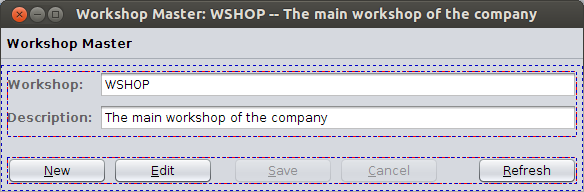
\includegraphics[width=0.65\textwidth]{parts/01-part/chapters/03-ui-construction/images/01-simple-master.png}
    }%

    \node [overlay, note=annotationbgcolor, callout absolute pointer={(4,0.8)}] at (7,0.8) 
    {
      \begin{minipage}{3cm}
       \tiny
       \textbf{Notification Panel}\newline
       An area where error and warning messages appear in a non-intrusive way.       
      \end{minipage}
    };
    
    \node [overlay, note=annotationbgcolor, callout absolute pointer={(4,-0.7)}] at (7,-0.7) 
    {
      \begin{minipage}{3cm}
       \tiny
       \textbf{Content Panel or Main Panel}\newline
       An area where UI controls such as property editors and buttons are placed.
      \end{minipage}
    };    
    
    \node [overlay, note=annotationbgcolor, callout absolute pointer={(-4,0)}] at (-7,0.5) 
    {
      \begin{minipage}{3cm}
       \tiny
       \textbf{Components Panel}\newline
       A container where property editors are added.
      \end{minipage}
    };
    
    \node [overlay, note=annotationbgcolor, callout absolute pointer={(-4,-1.0)}] at (-7,-0.5) 
    {
      \begin{minipage}{3cm}
       \tiny
       \textbf{Action Panel}\newline
       A container for CRUD and custom actions.
      \end{minipage}
    };    
    \end{tikzpicture}  
    
  \end{image}
  
  \paragraph{Layouting and Hints}
  
  Let's have a look at some layouting capabilities and the ways to provide the platform with additional hints when it comes to determining what kind of property editor should be used for a property.
  For this purpose, we shall continue using entity Workshop from our Rail domain.
  For out purpose let's consider that it has three properties -- the \emph{key} (serving as workshop's code), the \emph{desc} (its description) and property \emph{initial} that indicates whether workshop is the one where all rotables are collected for the very first time before being fitted onto wagons.
  %And let's walk through the design process of Workshop master.
  
  \subsubsection{Frame}
  
  \subsubsection{Factory}  
  
  
  \textbf{TODO}..............................
  
\subsection{Compound Masters}

  Compound masters should be used to represent a complex entity that consists of One-2-Many and One-2-One associations.
  The sole purpose to build a compound master is to have most if not all aspects of an entity editable in one place.
  Due to entity complexity caused by large number of properties and their complexity, it is necessary to logically split entity UI representation into several views.
  For example, entity \texttt{Wagon} has some primary properties such as its number and class.
  These can be grouped together on one view.
  At the same time its property \texttt{slots: Set<BogieSlot>}, which is a One-2-Many association, might be best represented on a separate view.
  Similarly, a One-2-One association such as property \texttt{techDetails: WagonTechDetails} is also best represented on a separate view.
  
  Such separation has dual purpose.
  On the one hand, user has clear visual separation between different aspect of the same entity while preserving everything as part of a single master view.
  On the other hand, this provide a way to optimise the fetch model in such way that not visible properties are not loaded until necessary, which helps reducing both database and network load.
  
  An important details here is that each master is associated with a particular instance of an entity object.
  The main view is associated directly with an entity, while other views are associated with complex properties (or set of properties) of the same entity instance.
  
  Structurally, compound masters are similar to simple masters.
  As the name suggests, instead of one model/view pair there are two and more such pairs.
  Each pair is associated with a tree menu item, which is located on the left side of each compound master view.
  Usually, the master model is associated with both the master view and the default view (aka main view).
  The master view holds the tree menu and the panel where menu specific views are displayed.
  

%\section{Configuration Management}


